% Fig. 2 kaynagi: mlp_engine boru hatti. Derleme:
%   pdflatex mlp_engine_pipeline.tex  ->  ../mlp_engine_pipeline.pdf olarak kopyala
% Makalede olceksiz girer (genislik <= \textwidth ~ 160 mm); yazilar 8 pt kalir.
\documentclass[tikz,border=2pt]{standalone}
\usepackage[T1]{fontenc}
\usepackage[scaled=0.92]{helvet}
\usepackage{amsmath}
\renewcommand{\familydefault}{\sfdefault}
\usetikzlibrary{positioning,arrows.meta,calc}

\definecolor{memfill}{HTML}{FFF4D6}\definecolor{memline}{HTML}{B8860B}
\definecolor{dpfill}{HTML}{E3F2E3}\definecolor{dpline}{HTML}{2E7D32}
\definecolor{axifill}{HTML}{E1ECF8}\definecolor{axiline}{HTML}{1F5FA8}
\definecolor{clkline}{HTML}{D2691E}

\tikzset{
  stg/.style={draw=dpline, fill=dpfill, rounded corners=2pt, line width=0.6pt,
              align=center, inner sep=2pt, text width=19.5mm, minimum height=18mm,
              font=\footnotesize},
  ff/.style={draw=memline, fill=memfill, rounded corners=1.5pt, line width=0.6pt,
             minimum width=5mm, minimum height=12mm, inner sep=0pt, font=\footnotesize},
  dat/.style={-{Latex[length=4pt]}, line width=0.6pt},
  clk/.style={line width=0.6pt, draw=clkline},
}
\newcommand{\st}[1]{{\color{black!60}#1}}

\begin{document}
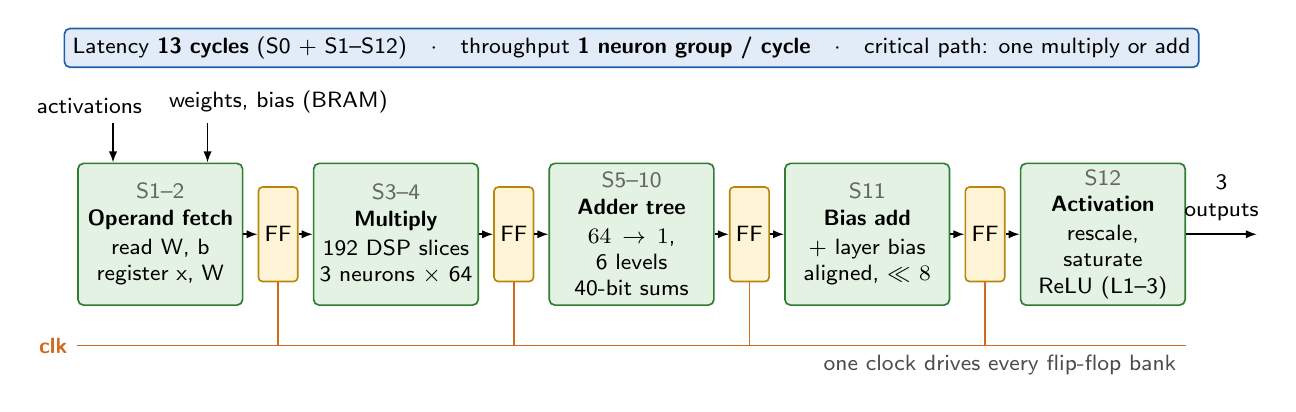
\begin{tikzpicture}[node distance=1.8mm]

\node[stg] (fetch) {\st{S1--2}\\\textbf{Operand fetch}\\[1pt]read W, b\\register x, W};
\node[ff, right=of fetch] (f1) {FF};
\node[stg, right=of f1] (mul) {\st{S3--4}\\\textbf{Multiply}\\[1pt]192 DSP slices\\3 neurons $\times$ 64};
\node[ff, right=of mul] (f2) {FF};
\node[stg, right=of f2] (add) {\st{S5--10}\\\textbf{Adder tree}\\[1pt]$64\to1$, 6 levels\\40-bit sums};
\node[ff, right=of add] (f3) {FF};
\node[stg, right=of f3] (bias) {\st{S11}\\\textbf{Bias add}\\[1pt]+ layer bias\\aligned, $\ll 8$};
\node[ff, right=of bias] (f4) {FF};
\node[stg, right=of f4] (act) {\st{S12}\\\textbf{Activation}\\[1pt]rescale, saturate\\ReLU (L1--3)};

\foreach \a/\b in {fetch/f1, f1/mul, mul/f2, f2/add, add/f3, f3/bias, bias/f4, f4/act}
  \draw[dat] (\a) -- (\b);

% girisler ustten, cikis sagdan
\coordinate (in1) at ($(fetch.north)+(-6mm,0)$);
\coordinate (in2) at ($(fetch.north)+(6mm,0)$);
\node[font=\footnotesize, anchor=south] (xin) at ($(in1)+(-3mm,5mm)$) {activations};
\node[font=\footnotesize, anchor=south] (win) at ($(in2)+(9mm,5mm)$) {weights, bias (BRAM)};
\draw[dat] (in1 |- xin.south) -- (in1);
\draw[dat] (in2 |- win.south) -- (in2);
\draw[dat] (act.east) -- ++(9mm,0) coordinate (oe);
\node[font=\footnotesize, align=center, anchor=south] at ($(act.east)!0.5!(oe)+(0,0.5mm)$) {3\\outputs};

% saat
\coordinate (cy) at ($(fetch.south)+(0,-5mm)$);
\draw[clk] (cy -| fetch.west) -- (cy -| act.east);
\node[font=\footnotesize\bfseries, text=clkline, anchor=east] at (cy -| fetch.west) {clk};
\foreach \f in {f1,f2,f3,f4} \draw[clk] (\f.south) -- (\f.south |- cy);
\node[font=\footnotesize, text=black!70, anchor=north east] at (cy -| act.east)
  {one clock drives every flip-flop bank};

% ozet bandi
\node[draw=axiline, fill=axifill, rounded corners=2pt, line width=0.6pt,
      font=\footnotesize, inner sep=3pt, anchor=south]
  at ($(mul.north)!0.5!(bias.north)+(0,12mm)$)
  {Latency \textbf{13 cycles} (S0 + S1--S12)\quad$\cdot$\quad
   throughput \textbf{1 neuron group / cycle}\quad$\cdot$\quad
   critical path: one multiply or add};

\end{tikzpicture}
\end{document}
